\documentclass[11pt,a4paper]{article}
\usepackage[margin=1.8cm]{geometry}
\usepackage{xcolor}
\usepackage{amssymb}
\usepackage{graphicx}
\usepackage[most]{tcolorbox}
\usepackage{array,tabularx,booktabs}
\usepackage{enumitem}
\usepackage{fontspec}
\usepackage{polyglossia}
\setdefaultlanguage{french}
\setotherlanguage{arabic}
\setmainfont{DejaVu Serif}
\newfontfamily\arabicfont[Script=Arabic,Scale=1.05]{DejaVu Sans}
\newfontfamily\arabicfontsf[Script=Arabic,Scale=1.05]{DejaVu Sans}
\graphicspath{{img/}}
\setlength{\parindent}{0pt}
\setlength{\parskip}{4pt}
\renewcommand{\arraystretch}{1.35}
\setlist{itemsep=2pt,topsep=3pt}

\definecolor{bleu}{HTML}{2E5C9A}
\definecolor{vert}{HTML}{2E7D32}
\definecolor{rouge}{HTML}{C62828}
\definecolor{orange}{HTML}{E65100}
\definecolor{gris}{HTML}{455A64}
\definecolor{violet}{HTML}{6A1B9A}
\definecolor{teal}{HTML}{00695C}

\newtcolorbox{carte}{colback=bleu!6,colframe=bleu,title=Où on est sur la carte,fonttitle=\bfseries}
\newtcolorbox{examen}{colback=vert!6,colframe=vert,title=Phrases d'examen à connaître (en français),fonttitle=\bfseries}
\newtcolorbox{piege}{colback=rouge!5,colframe=rouge,title=Pièges des examens,fonttitle=\bfseries}
\newtcolorbox{resume}{colback=orange!6,colframe=orange,title=Résumé en 3 phrases,fonttitle=\bfseries}
\newtcolorbox{note}{colback=gris!6,colframe=gris,title=Note / Astuce,fonttitle=\bfseries}
\newtcolorbox{alerte}{colback=violet!5,colframe=violet,title=Alerte : les sources ne sont pas d'accord,fonttitle=\bfseries}
\newtcolorbox{exemple}{colback=teal!5,colframe=teal,title=Exemple,fonttitle=\bfseries}

\newcommand{\ar}[1]{\textarabic{#1}}
\newcommand{\fr}[1]{\textfrench{#1}}
\newcommand{\vrai}{\textcolor{vert}{\textbf{VRAI}}}
\newcommand{\faux}{\textcolor{rouge}{\textbf{FAUX}}}
\newcommand{\partie}[1]{\newpage\section*{#1}\addcontentsline{toc}{section}{#1}}

\begin{document}

%======================================================================
\begin{center}
{\LARGE\bfseries Systèmes de Production}\\[4pt]
{\Large Chapitre 2 : la pyramide productique}\\[4pt]
{\large Fiche de révision (arabe + français)}\\[2pt]
{\small Basée sur le cours (BARABAS), le TD1 et les tests 2022-23, 2023-24, 2024-25}
\end{center}

\section*{0. La carte du chapitre}

\par\begin{Arabic}
\textbf{الفكرة ديال الفصل 2 فجملة وحدة:} كيفاش مشينا من \textbf{ماكينات معزولة} حتى لـ\textbf{معمل كامل مربوط وذكي}؟
\end{Arabic}

\begin{center}
\begin{tabularx}{\linewidth}{c >{\raggedleft\arraybackslash}X l c}
\toprule
\textbf{Partie} & \ar{\textbf{السؤال}} & \textbf{Titre} & \textbf{Questions} \\
\midrule
1 & \ar{شنو هي الأتمتة؟ وشنو هي الأنظمة المرنة؟} & Bases + FMS, cellule, atelier & 4 \\
2 & \ar{كيفاش كيتنظم المعمل فـ5 طوابق؟} & Pyramide CIM + réseaux & 8 \\
3 & \ar{شنو كيدير كل برنامج؟} & SCADA / MES / ERP & 8 \\
4 & \ar{كيفاش المعمل يتبدل بسرعة؟} & RMS + Plug and Produce & 6 \\
5 & \ar{المعمل الذكي والمستقبل} & Industrie 4.0, CPS, pyramide aplatie & 13 \\
\bottomrule
\end{tabularx}
\end{center}

\begin{tcolorbox}[colback=bleu!4,colframe=bleu,title=La chaîne logique du chapitre,fonttitle=\bfseries]
\centering
\textbf{Partie 1} (machines flexibles) $\longrightarrow$ \textbf{Partie 2} (on les relie : CIM) $\longrightarrow$ \textbf{Partie 3} (les logiciels de chaque étage)\\[3pt]
$\longrightarrow$ \textbf{Partie 4} (on les reconfigure) $\longrightarrow$ \textbf{Partie 5} (tout connecté : Industrie 4.0)
\par\begin{Arabic}
\centering
ماكينات ← ربط ← برامج ← مرونة ← معمل ذكي
\end{Arabic}
\end{tcolorbox}

\subsection*{Poids du chapitre 2 dans les examens}
\begin{center}
\begin{tabular}{lccc}
\toprule
\textbf{Source} & \textbf{Total} & \textbf{Chapitre 2} & \textbf{Chapitre 1} \\
\midrule
TD1 & 37 & 13 & 24 \\
Test 2022-23 & 20 & 3 & 17 \\
Test 2023-24 & 38 & 16 & 22 \\
Test 2024-25 & 22 & 7 & 15 \\
\midrule
\textbf{Total} & \textbf{117} & \textbf{39} & \textbf{78} \\
\bottomrule
\end{tabular}
\end{center}
\par\begin{Arabic}
\textbf{يعني:} الفصل 2 هو \textbf{التلت} ديال الأسئلة (39 من 117)، ولكن فامتحان 2023-24 كان \textbf{تقريبا النص} (16 من 38).
\end{Arabic}

\subsection*{Comment lire cette fiche}
\begin{itemize}
\item \textcolor{bleu}{\textbf{Bleu}} : où on est et à quoi sert la partie.
\item \textcolor{vert}{\textbf{Vert}} : phrases exactes des examens (VRAIES).
\item \textcolor{rouge}{\textbf{Rouge}} : pièges (VRAI / FAUX).
\item \textcolor{gris}{\textbf{Gris}} : notes et astuces.
\item \textcolor{violet}{\textbf{Violet}} : alertes quand le TD, le cours et les tests se contredisent.
\item \textcolor{orange}{\textbf{Orange}} : résumé à relire la veille de l'examen.
\end{itemize}

\begin{alerte}
\textbf{Règle adoptée pour les conflits :} on suit les \textbf{corrigés des tests} quand ils contredisent les annotations du TD. Les points concernés sont signalés par une alerte violette et \textbf{à confirmer avec le prof}.
\end{alerte}

%======================================================================
\partie{Partie 1 : Les bases et les systèmes flexibles}

\begin{carte}
\textbf{Partie 1} $\rightarrow$ 2 $\rightarrow$ 3 $\rightarrow$ 4 $\rightarrow$ 5
\par\begin{Arabic}
\textbf{الدور ديال هاد الجزء:} نفهمو شنو هي الأتمتة، كيفاش تطورات الصناعة، ونعرفو الأنواع ديال الأنظمة المرنة.
\end{Arabic}
\end{carte}

\subsection*{1. Deux mots à connaître}
\begin{center}
\begin{tabularx}{\linewidth}{l >{\raggedleft\arraybackslash}X}
\toprule
\textbf{Mot} & \ar{\textbf{بالدارجة}} \\
\midrule
Automatisation & \ar{كنخليو الماكينات تدير الخدمة بلاصة الإنسان} \\
Productique & \ar{كاع الوسائل والطرق (إعلاميات، أوتوماتيك، ميكانيك، إلكترونيك) باش نحسنو الأداء ديال المعمل} \\
\bottomrule
\end{tabularx}
\end{center}
\textbf{But final de la productique :} une usine \textbf{intelligente, autonome, connectée, durable}.

\textbf{Degrés d'automatisation :} (1) production de masse automatisée avec machines \textbf{spécialisées} (très efficaces, mais un seul produit) ; (2) \textbf{automatisation flexible} (la machine s'adapte à plusieurs produits) ; (3) machines \textbf{reconfigurables}, robots programmables, systèmes \textbf{intégrés}.

\begin{note}
\textbf{Industrie 4.0 = digitalisée + décisionnelle + autonome.}
\end{note}

\subsection*{2. L'historique en 4 étapes}
\begin{center}
\begin{tabularx}{\linewidth}{l l X}
\toprule
\textbf{Étape} & \textbf{Époque} & \textbf{Caractéristiques} \\
\midrule
Automatisation ponctuelle & années 60 & une machine ou une fonction précise ; machines dédiées, \textbf{non flexibles} \\
Îlots d'automatisation & ensuite & MOCN, manutention et stockage automatiques, \textbf{CFAO} (CAO + EFAO + FAO), cellules flexibles d'usinage \\
Production intégrée & ensuite & on relie les îlots en un tout cohérent = \textbf{pyramide CIM} \\
Industrie 4.0 & aujourd'hui & \textbf{CPS}, \textbf{Digital Twin}, \textbf{pyramide aplatie} grâce à Internet \\
\bottomrule
\end{tabularx}
\end{center}
\begin{note}
\par\begin{Arabic}
\textbf{باش تتفكر:} نقطة معزولة ← جزر (\fr{îlots}) ← جزر مربوطة ← كلشي مربوط.
\end{Arabic}
\end{note}

\subsection*{3. Le FMS (Flexible Manufacturing System)}
\par\begin{Arabic}
نظام تصنيع \textbf{مرن}: كيصنع بزاف ديال أنواع القطع بلا ما نبدلو كلشي \textbf{باليد}.
\end{Arabic}
\begin{center}
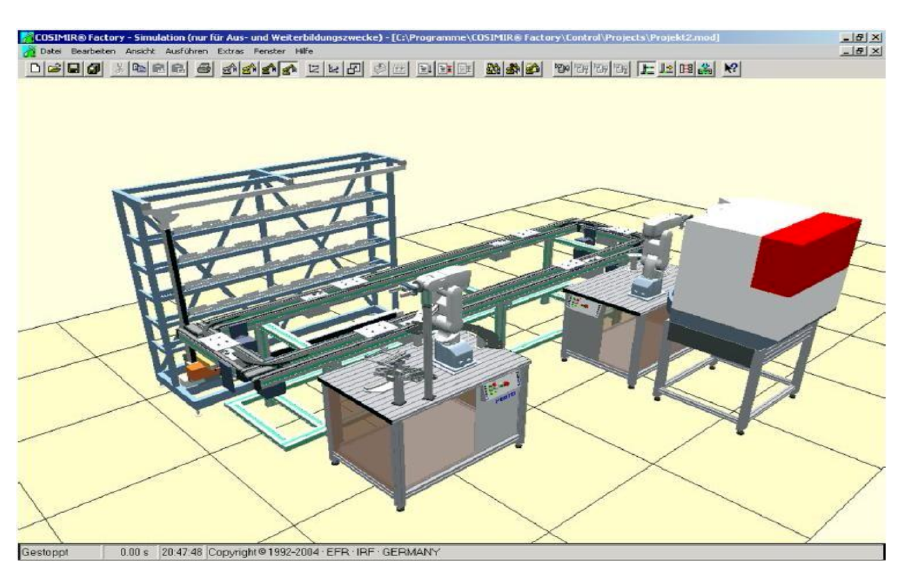
\includegraphics[width=0.7\linewidth]{ch2_fms}\\
\small Un FMS : rayonnage (stockage), convoyeur (transport), robots (manipulation), machine-outil (production)
\end{center}
\begin{center}
\begin{tabularx}{\linewidth}{l X >{\raggedright\arraybackslash}X}
\toprule
\textbf{Composant} & \textbf{Rôle} & \textbf{Détails} \\
\midrule
Moyens de production & transformer les produits entrants en sortants & les machines \\
Moyens de stockage & casiers desservis par un dispositif de stockage / déstockage & \textbf{ASRS} \\
Moyens de transport & transporter la matière dans l'atelier & lignes de transfert, convoyeurs, chariots filoguidés, \textbf{AGV} \\
Robots et manipulateurs & déplacer une pièce (chargement, déchargement) & \\
Logiciels de pilotage & \textbf{coordination} entre les machines & le « cerveau » du FMS \\
\bottomrule
\end{tabularx}
\end{center}

\subsection*{4. Les 4 systèmes : taille des séries et nombre de variantes}
\begin{center}
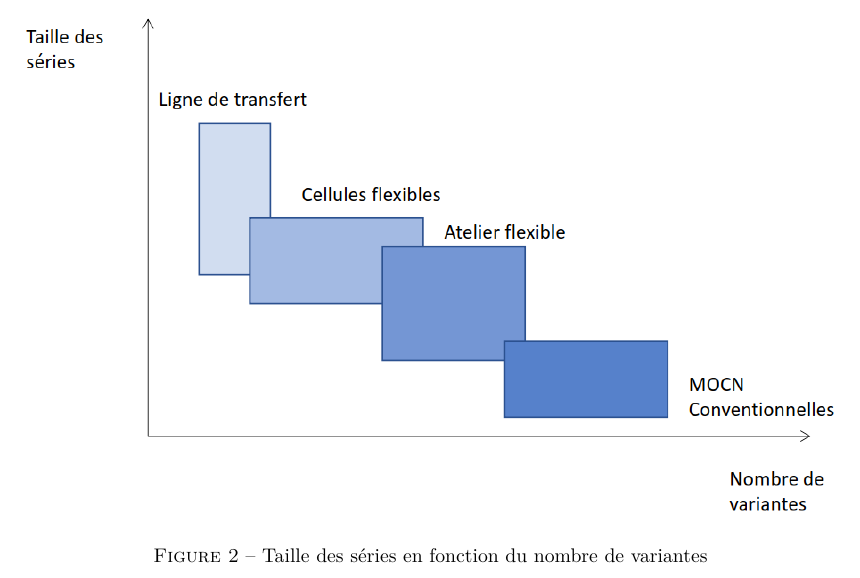
\includegraphics[width=0.6\linewidth]{ch2_series_variantes}
\end{center}
\begin{center}
\begin{tabularx}{\linewidth}{l >{\raggedleft\arraybackslash}X l l}
\toprule
\textbf{Système} & \ar{\textbf{بالدارجة}} & \textbf{Séries} & \textbf{Variantes} \\
\midrule
Ligne de transfert & \ar{ماكينات أوتوماتيكية مربوطة بنقل؛ القطعة كتمشي بين المحطات \textbf{بلا تدخل بشري}} & très grandes & peu \\
Cellule flexible & \ar{\textbf{عدة} ماكينات CNC + روبو + كمبيوتر مركزي} & moyennes & moyennes \\
Atelier flexible & \ar{مجموعة \fr{cellules flexibles} مربوطة، مسيرة بالحاسوب} & plus petites & beaucoup \\
MOCN conventionnelles & \ar{ماكينات CNC \textbf{معزولة}} & petites & grande variété \\
\bottomrule
\end{tabularx}
\end{center}
\begin{note}
\textbf{À retenir :} plus on est \textbf{flexible}, moins on produit en grande série, et inversement. La ligne de transfert est très efficace pour un seul produit en masse, mais elle est \textbf{rigide}.
\end{note}

\begin{examen}
\begin{itemize}
\item « Un système de fabrication flexible contient un système de \textbf{manutention automatisé}, un \textbf{stockage automatisé} et un \textbf{pilotage par ordinateur centralisé}. »
\item « L'automatisation flexible est capable de \textbf{réduire les délais} de fabrication et offre l'inclusion d'une \textbf{variété de produits}. »
\item « Un FMS est capable de produire quelques \textbf{familles de pièces} en utilisant la \textbf{technologie de groupe}. »
\item « Un FMS se distingue par l'\textbf{adaptation rapide} pour produire une \textbf{diversité de produits}. »
\item « Un FMS est nécessaire pour répondre à une forte demande de \textbf{personnalisation}. »
\item « Une cellule flexible d'usinage \textbf{utilise la technologie de groupe}. »
\item « Pour produire une \textbf{grande variété}, il faut opter pour un système flexible \textbf{FMS}. »
\item « Un système automatisé, flexible et intégré dans une pyramide CIM permet d'\textbf{optimiser la production, les contrôles et la gestion de l'information}. »
\end{itemize}
\end{examen}
\begin{piege}
\begin{itemize}
\item « Un FMS produit \textbf{une seule variante} de produit. » \faux
\item « Un FMS se distingue par l'\textbf{absence de supervision humaine}. » \faux
\item « Un FMS : reconfiguration automatique via technologies de communication \textbf{propriétaire}. » \faux \ \ar{(هادا \fr{Plug and Produce}، وكيستعمل \fr{standards})}
\item « Une cellule flexible est composée de \textbf{machines dédiées et de lignes de transfert}. » \faux
\item « Une cellule flexible est \textbf{plus flexible} qu'un atelier flexible. » \faux \ \ar{(العكس)}
\item « Réduire la flexibilité et augmenter la production en masse. » \faux
\end{itemize}
\end{piege}
\begin{alerte}
Test 2022-23 : « Une cellule flexible contient \textbf{$n=1$ à $4$} machines CNC » est coché \textbf{vrai}, alors que le cours dit seulement « \textbf{plusieurs} machines CNC ». Si la phrase tombe, coche-la.
\end{alerte}

\begin{resume}
\begin{enumerate}
\item Automatisation : machines isolées $\rightarrow$ îlots $\rightarrow$ intégré (CIM) $\rightarrow$ Industrie 4.0.
\item FMS = production, stockage (ASRS), transport (AGV), robots, pilotage ; flexible, technologie de groupe.
\item Ligne de transfert (grandes séries) $\rightarrow$ cellule $\rightarrow$ atelier $\rightarrow$ MOCN (grande variété).
\end{enumerate}
\end{resume}

\subsection*{Mini-QCM}
\begin{enumerate}
\item Un FMS se distingue par : (a) une seule variante (b) l'adaptation rapide pour produire une diversité de produits (c) l'absence de supervision humaine
\item Une cellule flexible d'usinage : (a) machines dédiées + lignes de transfert (b) utilise la technologie de groupe (c) plus flexible qu'un atelier flexible
\item Très grandes séries, peu de variantes : (a) MOCN (b) atelier flexible (c) ligne de transfert
\item Le « cerveau » du FMS : (a) les robots (b) le logiciel de pilotage (c) le stockage
\end{enumerate}
{\small\textit{Réponses : 1-b, 2-b, 3-c, 4-b.}}

%======================================================================
\partie{Partie 2 : La pyramide CIM et les réseaux industriels}

\begin{carte}
1 \checkmark\ $\rightarrow$ \textbf{Partie 2} $\rightarrow$ 3 $\rightarrow$ 4 $\rightarrow$ 5
\par\begin{Arabic}
\textbf{الدور ديال هاد الجزء:} الجزر كيتربطو. دابا نشوفو \textbf{كيفاش كيتنظمو}: \textbf{5 طوابق}، وكل طابق كيهضر مع اللي فوقو وتحتو بواسطة \textbf{شبكة}.
\end{Arabic}
\end{carte}

\subsection*{1. La pyramide CIM}
\textbf{CIM = Computer Integrated Manufacturing.}
\par\begin{Arabic}
تنظيم \textbf{هرمي} (\fr{hiérarchique}) ديال الأنظمة المعلوماتية والتسيير فالمعمل. بحال عمارة من 5 طوابق.
\end{Arabic}
\begin{center}
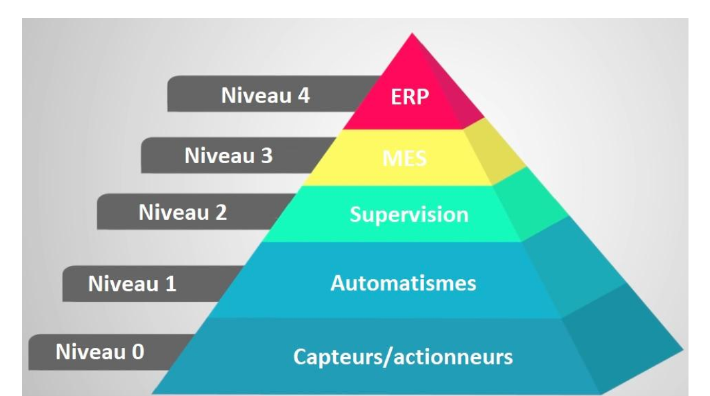
\includegraphics[width=0.55\linewidth]{ch2_pyramide_cim}
\end{center}
\begin{center}
\begin{tabularx}{\linewidth}{c l X >{\raggedleft\arraybackslash}X}
\toprule
\textbf{Niveau} & \textbf{Nom} & \textbf{Rôle} & \ar{\textbf{بالدارجة}} \\
\midrule
4 & \textbf{ERP} & gérer toute l'entreprise (achats, stocks, ventes, comptabilité, RH) & \ar{تسيير} \\
3 & \textbf{MES} & exécuter et suivre la production en temps réel & \ar{تنفيذ} \\
2 & \textbf{SCADA} (supervision) & visualiser et superviser les processus & \ar{مراقبة} \\
1 & \textbf{Automatismes} & commander les machines & \ar{تحكم} \\
0 & \textbf{Capteurs / actionneurs} & interagir avec le monde physique & \ar{حس} \\
\bottomrule
\end{tabularx}
\end{center}
\begin{note}
\textbf{Règle de lecture :} plus on \textbf{monte}, plus on fait de la \textbf{décision et de la gestion}. Plus on \textbf{descend}, plus on est proche de la \textbf{machine} et du \textbf{temps réel}.
\par\begin{Arabic}
\textbf{الترتيب من تحت لفوق:} \fr{Capteurs → Automates → SCADA → MES → ERP}
\end{Arabic}
\end{note}

\begin{examen}
\begin{itemize}
\item « La pyramide CIM est un \textbf{modèle hiérarchique} de l'automatisation intégrée d'une usine de fabrication. »
\item « La pyramide CIM décrit l'automatisation d'une usine et comporte \textbf{cinq niveaux}. »
\item « La pyramide CIM est utilisée pour \textbf{organiser les activités} dans un système de production intégré. »
\item « CIM = \textbf{Computer Integrated Manufacturing}. »
\end{itemize}
\end{examen}
\begin{piege}
« Un modèle de gestion de la qualité » \faux \quad « Un outil de mesure de la variabilité des processus » \faux \quad « Améliorer la flexibilité des machines » \faux \quad « Classer les produits selon leur complexité » \faux
\end{piege}

\subsection*{2. La machine (niveau 1)}
La machine est l'\textbf{entité élémentaire} d'un FMS : une \textbf{partie opérative} (axes, moteurs, outils) et une \textbf{partie commande} (le contrôleur). Le contrôleur d'une MOCN assure 3 fonctions : \textbf{programmation, commande, visualisation}, avec deux aspects : l'\textbf{automate} (ses entrées-sorties commandent les axes) et le \textbf{calculateur} (écrire les programmes : RAM, microprocesseur, clavier, écran).

\textbf{Langage :} \textbf{APT} (Automatic Programmed Tools), connu sous le nom de \textbf{code G}, normalisé ISO = \textbf{code ISO}. Un logiciel \textbf{FAO} génère automatiquement les programmes de commande numérique. \textit{(Peu testé.)}

\subsection*{3. Les 4 réseaux locaux industriels (RLI)}
\textbf{RLI :} réseau local utilisé dans une usine pour connecter les machines : commande, supervision, conduite, maintenance, gestion.
\begin{center}
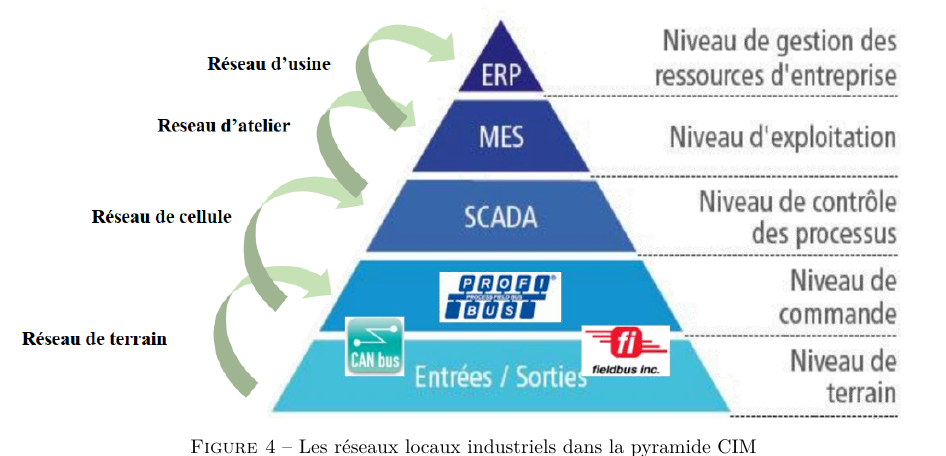
\includegraphics[width=0.75\linewidth]{ch2_reseaux_rli}
\end{center}
\par\begin{Arabic}
\textbf{القاعدة:} شبكة وحدة \textbf{بين كل جوج طوابق}، وكتاخد \textbf{اسم الطابق الأعلى}.
\end{Arabic}
\begin{center}
\begin{tabularx}{\linewidth}{l c X}
\toprule
\textbf{Réseau} & \textbf{Entre} & \textbf{Il connecte\ldots} \\
\midrule
\textbf{Terrain} & $0 \leftrightarrow 1$ & capteurs et actionneurs $\leftrightarrow$ \textbf{automates} (CAN bus, Profibus, Fieldbus ; les tests ajoutent \textbf{CANopen} et \textbf{AS-i}) \\
\textbf{Cellule} & $1 \leftrightarrow 2$ & les \textbf{automates} $\leftrightarrow$ le coordinateur \textbf{SCADA} \\
\textbf{Atelier} & $2 \leftrightarrow 3$ & les cellules $\leftrightarrow$ le \textbf{MES} (Wonderware, FactoryCast…) \\
\textbf{Usine} & $3 \leftrightarrow 4$ & les coordinateurs $\leftrightarrow$ services : bureau d'études, méthodes, approvisionnement \\
\bottomrule
\end{tabularx}
\end{center}

\subsection*{4. Le grand classique : test 2024-25 Q15}
\begin{center}
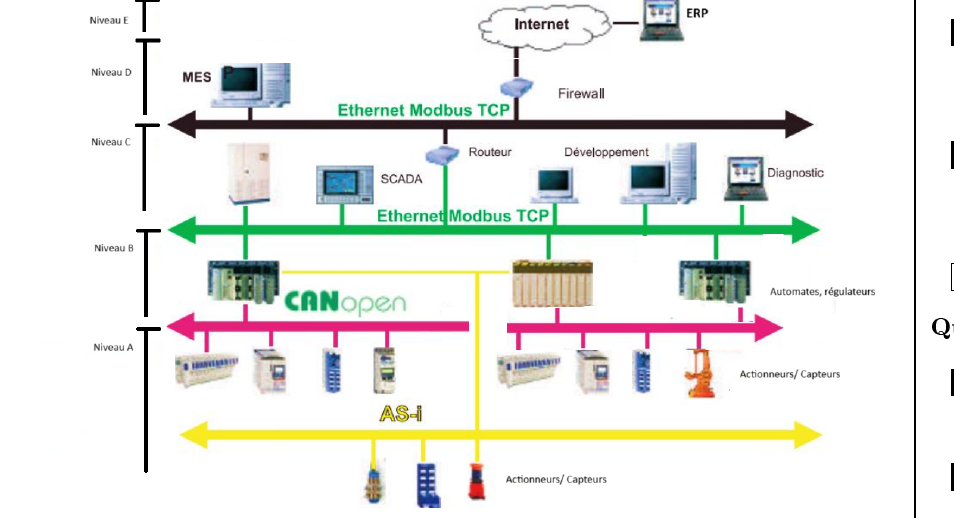
\includegraphics[width=0.8\linewidth]{ch2_fms_niveaux_examen}
\end{center}
\begin{center}
\begin{tabular}{llll}
\toprule
\textbf{Niveau} & \textbf{Étage CIM} & \textbf{Éléments} & \textbf{Protocole} \\
\midrule
\textbf{A} & terrain & capteurs et actionneurs & \textbf{CANopen, AS-i} \\
\textbf{B} & machine & automates et contrôle & \textbf{Ethernet Modbus TCP} \\
\textbf{C} & cellule & \textbf{SCADA} supervision & \textbf{Ethernet Modbus TCP} \\
\textbf{D} & atelier & \textbf{MES} & \textbf{Ethernet Modbus TCP} \\
\textbf{E} & usine & \textbf{ERP}, serveur cloud & \\
\bottomrule
\end{tabular}
\end{center}
\begin{note}
\textbf{Ethernet Modbus TCP} apparaît à \textbf{3 niveaux} (B, C, D). \textbf{CANopen et AS-i} : seulement au niveau \textbf{A}.
\end{note}

\subsection*{5. Les pièges}
\begin{piege}
\begin{itemize}
\item « Le \textbf{réseau de cellule} connecte les \textbf{capteurs et actionneurs} aux systèmes de supervision. » \faux \ \ar{(هادا \fr{réseau de terrain})}
\item « 1 = réseau 5G, 2 = 4G, 3 = 3G » \faux \qquad « 1 = ERP, 2 = SCADA, 3 = capteurs » \faux
\item Test 2022-23 Q6 : \textbf{1 = réseau usine, 2 = réseau cellule, 3 = réseau terrain} \vrai
\end{itemize}
\end{piege}

\subsection*{6. Associer des éléments aux niveaux (TD Q28)}
\begin{center}
\begin{tabularx}{\linewidth}{c X}
\toprule
\textbf{Niveau} & \textbf{Éléments} \\
\midrule
\textbf{4} & ERP ; gestion des produits et des stocks ; gestion des approvisionnements \\
\textbf{3} & MES ; ordre de fabrication ; allocation de ressources (machine, poste, opérateur, tâches) ; traçabilité ; localisation des produits en stock ; mouvements physiques et gestion des lots \\
\textbf{2} & SCADA ; états du process ; états des ressources ; aléas \\
\textbf{1} & automate, PLC, PID \\
\textbf{0} & capteurs ; actionneurs ; vérin hydraulique ; accéléromètre \\
\bottomrule
\end{tabularx}
\end{center}
\begin{alerte}
Le cours dit que le \textbf{MES} détecte les \textbf{aléas} et réagit vite, mais la correction du TD les place au niveau \textbf{2 (SCADA)}. À confirmer avec le prof.
\end{alerte}

\begin{resume}
\begin{enumerate}
\item 5 niveaux (0 à 4) : capteurs $\rightarrow$ automates $\rightarrow$ SCADA $\rightarrow$ MES $\rightarrow$ ERP. En haut : gestion ; en bas : temps réel.
\item 4 réseaux : terrain ($0\leftrightarrow1$), cellule ($1\leftrightarrow2$), atelier ($2\leftrightarrow3$), usine ($3\leftrightarrow4$).
\item Ethernet Modbus TCP aux niveaux B, C, D ; CANopen et AS-i au niveau A.
\end{enumerate}
\end{resume}

\subsection*{Mini-QCM}
\begin{enumerate}
\item Combien de niveaux a la pyramide CIM ? (a) 3 (b) 4 (c) 5
\item Le réseau de cellule relie : (a) capteurs et automates (b) automates et SCADA (c) MES et ERP
\item CANopen et AS-i se trouvent au niveau : (a) A (terrain) (b) C (cellule) (c) E (usine)
\item Le SCADA est au niveau : (a) 1 (b) 2 (c) 3
\end{enumerate}
{\small\textit{Réponses : 1-c, 2-b, 3-a, 4-b.}}

%======================================================================
\partie{Partie 3 : SCADA, MES et ERP}

\begin{carte}
1, 2 \checkmark\ $\rightarrow$ \textbf{Partie 3} $\rightarrow$ 4 $\rightarrow$ 5
\par\begin{Arabic}
\textbf{الدور ديال هاد الجزء:} نشوفو \textbf{شنو كيدير} كل برنامج من الثلاثة الفوقانيين: \textbf{SCADA} (2)، \textbf{MES} (3)، \textbf{ERP} (4). وهنا بالضبط كيغلطو بزاف فالامتحان.
\end{Arabic}
\end{carte}

\subsection*{1. Trois systèmes, trois rôles}
\begin{exemple}
\par\begin{Arabic}
\textbf{مثال المطعم:} \textbf{ERP} = مدير المطعم (كيشري، الميزانية، الأجور) \quad|\quad \textbf{MES} = رئيس الطباخين (كياخد الطلبية، كيوزع الخدمة، كيسجل شنو تطبخ) \quad|\quad \textbf{SCADA} = الشاشة فالمطبخ (كتبين شنو كيوقع).
\end{Arabic}
\end{exemple}
\begin{center}
\begin{tabularx}{\linewidth}{l c l X}
\toprule
\textbf{Système} & \textbf{Niveau} & \textbf{Mot-clé} & \textbf{Rôle} \\
\midrule
\textbf{ERP} & 4 & \textbf{Gestion} & gérer toute l'entreprise \\
\textbf{MES} & 3 & \textbf{Exécution + traçabilité} & exécuter et suivre la production \\
\textbf{SCADA} & 2 & \textbf{Supervision} & visualiser et superviser les machines \\
\bottomrule
\end{tabularx}
\end{center}

\subsection*{2. SCADA (Supervisory Control and Data Acquisition)}
Il sert à : \textbf{représenter graphiquement} les machines et visualiser leur état (écrans de supervision) ; \textbf{communiquer} avec les systèmes de contrôle-commande (API, SNCC…) ; \textbf{déporter et centraliser} le pilotage des machines ; \textbf{collecter les données} et gérer une base de données temps réel.
\begin{examen}
\begin{itemize}
\item « Permet d'assurer la fonction \textbf{collecte et archivage des données}. »
\item « Permet de \textbf{superviser en temps réel} les moyens de production. »
\item « Un logiciel qui \textbf{pilote en temps réel} les moyens de production. » \ (test 2023-24 Q24)
\end{itemize}
\end{examen}
\begin{piege}
« Traçabilité de la production » \faux \ \ar{(\fr{MES})} \quad « Planification globale des capacités » \faux \ \ar{(\fr{ERP})} \quad « Gestion de la production » \faux \quad « Gestion des stocks » \faux
\end{piege}

\subsection*{3. MES (Manufacturing Execution System)}
Logiciel \textbf{intermédiaire} entre l'ERP (niveau de planification) et l'atelier (SCADA, machines, automates, opérateurs). Il assure la \textbf{coordination, le suivi et l'optimisation en temps réel} des activités de production.

\begin{note}
\textbf{4 mots à retenir pour le MES :} \textbf{exécute les OF} \;|\; \textbf{ordonnancement détaillé} \;|\; \textbf{traçabilité} \;|\; \textbf{collecte et traite les données}.
\end{note}
\begin{examen}
\begin{itemize}
\item « Permet d'assurer un \textbf{ordonnancement détaillé} de la production. »
\item « Permet d'assurer la fonction \textbf{traçabilité} de la production. »
\item « Il \textbf{exécute les ordres de fabrication} dans l'atelier de production. »
\item « Il \textbf{collecte et traite les données} de production et assure la traçabilité. »
\item « Assure le \textbf{lien} entre le système informatique de \textbf{gestion} et le système de \textbf{contrôle commande}. »
\item « Permet la \textbf{gestion des informations} liées à la production. »
\item Le MES est le logiciel de \textbf{pilotage d'atelier}.
\end{itemize}
\end{examen}
\begin{piege}
\begin{itemize}
\item « Il assure la \textbf{supervision} des machines de production. » \faux
\item « Il gère la \textbf{comptabilité} de l'entreprise. » \faux
\item « Il assure un \textbf{temps de réponse de l'ordre de la seconde}. » \faux
\item « Réalise un \textbf{pilotage en temps réel} de l'atelier. » \faux \ (test 2023-24 Q21)
\end{itemize}
\end{piege}

\subsection*{4. ERP (Enterprise Resource Planning)}
Système de gestion \textbf{intégré} qui pilote l'ensemble des ressources et processus de l'entreprise grâce à \textbf{une base de données unique} et des modules interconnectés : achats, production, stocks, ventes, comptabilité, RH.

\textbf{Objectifs :} centraliser l'information dans une base unique ; éviter les doublons et incohérences ; améliorer la coordination entre départements ; optimiser coûts, délais et qualité.
\begin{examen}
« \textbf{Gérer les ressources de l'entreprise}, y compris les finances, la logistique et les ressources humaines. »
\end{examen}
\begin{piege}
« Assurer la fonction \textbf{traçabilité} de la production » \faux \quad « \textbf{Planifier la production détaillée} » \faux \ \ar{(هادا \fr{MES})}
\end{piege}

\subsection*{5. Le dialogue ERP – MES – Atelier}
\begin{center}
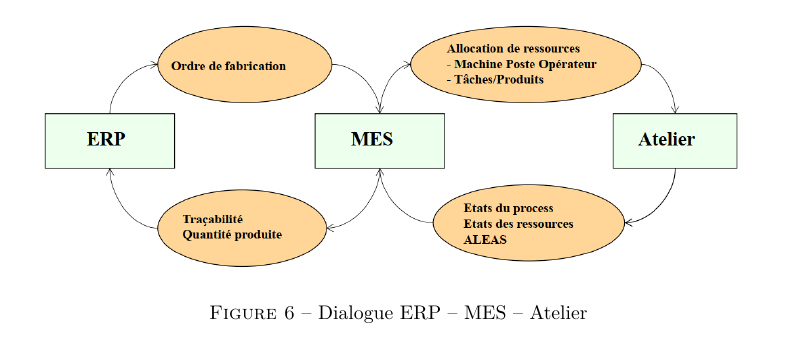
\includegraphics[width=0.7\linewidth]{ch2_dialogue_erp_mes}
\end{center}
\begin{center}
\begin{tabularx}{\linewidth}{l X}
\toprule
\textbf{De $\rightarrow$ vers} & \textbf{Ce qui circule} \\
\midrule
ERP $\rightarrow$ MES & \textbf{ordre de fabrication} \\
MES $\rightarrow$ ERP & \textbf{traçabilité}, \textbf{quantité produite} \\
MES $\rightarrow$ atelier & \textbf{allocation de ressources} (machine, poste, opérateur, tâches / produits) \\
atelier $\rightarrow$ MES & \textbf{états du process}, \textbf{états des ressources}, \textbf{aléas} \\
\bottomrule
\end{tabularx}
\end{center}
\textbf{Aléas} = imprévus (panne, retard, rupture de matière) = \textbf{gaspillage}. Le MES sert à les détecter et à réagir vite.

\subsection*{6. Système d'information : opérationnel vs décisionnel}
\begin{center}
\begin{tabularx}{\linewidth}{l X l}
\toprule
\textbf{Type} & \textbf{Rôle} & \textbf{Niveaux} \\
\midrule
Opérationnel & capter les informations et opérations pour \textbf{faire fonctionner} le système & niveaux bas \\
Décisionnel & aider à \textbf{prendre des décisions} (système décisionnel intelligent) & niveaux hauts (MES, ERP) \\
\bottomrule
\end{tabularx}
\end{center}

\begin{alerte}
\begin{itemize}
\item MES « superviser en temps réel les moyens de production » : le \textbf{TD} le coche vrai, le \textbf{test 2023-24 Q21} le refuse. \textbf{Décision : on suit le test (faux).}
\item « Supervision / temps réel » $\Rightarrow$ \textbf{SCADA}. « Ordonnancement / traçabilité / OF » $\Rightarrow$ \textbf{MES}. « Finances / RH / logistique » $\Rightarrow$ \textbf{ERP}.
\item Test 2022-23 Q3 : « grâce à la pyramide aplatie, on n'a plus besoin de l'ERP et du MES » \faux.
\end{itemize}
\end{alerte}

\begin{resume}
\begin{enumerate}
\item ERP = gestion de l'entreprise (finances, RH, logistique) ; MES = exécution + ordonnancement détaillé + traçabilité ; SCADA = supervision + collecte des données.
\item ERP $\rightarrow$ MES : OF ; MES $\rightarrow$ ERP : traçabilité ; MES $\rightarrow$ atelier : allocation ; atelier $\rightarrow$ MES : états + aléas.
\item Le MES ne « supervise » pas (selon les tests) et la pyramide aplatie ne supprime ni l'ERP ni le MES.
\end{enumerate}
\end{resume}

\subsection*{Mini-QCM}
\begin{enumerate}
\item « Ordonnancement détaillé » et « traçabilité » : (a) SCADA (b) MES (c) ERP
\item « Gérer les finances, la logistique et les RH » : (a) SCADA (b) MES (c) ERP
\item Qui envoie l'ordre de fabrication au MES ? (a) l'ERP (b) le SCADA (c) l'atelier
\item « Collecte et archivage des données », « superviser » : (a) SCADA (b) MES (c) ERP
\end{enumerate}
{\small\textit{Réponses : 1-b, 2-c, 3-a, 4-a.}}

%======================================================================
\partie{Partie 4 : RMS et Plug and Produce}

\begin{carte}
1, 2, 3 \checkmark\ $\rightarrow$ \textbf{Partie 4} $\rightarrow$ 5
\par\begin{Arabic}
\textbf{الدور ديال هاد الجزء:} الـ \fr{FMS} مرن، ولكن عندو حدود. نشوفو كيفاش \textbf{نتجاوزوها} بنظام \textbf{قابل لإعادة التشكيل}.
\end{Arabic}
\end{carte}

\subsection*{1. Pourquoi dépasser le FMS ?}
Le FMS repose sur le concept du CIM et apporte de la flexibilité, mais il \textbf{atteint ses limites} quand la demande varie \textbf{souvent et de façon imprévisible}, en diversité de produits comme en volumes.
\par\begin{Arabic}
\fr{FMS} ما مزيانش مع التغييرات \textbf{الكثيرة وغير المتوقعة}.
\end{Arabic}

\subsection*{2. RMS (Reconfigurable Manufacturing System)}
Système conçu pour s'adapter \textbf{rapidement} aux changements de produits ou de volumes grâce à des \textbf{modules reconfigurables} (machines, logiciels, outils). C'est une \textbf{évolution du FMS vers plus d'agilité}.
\begin{exemple}
\par\begin{Arabic}
\textbf{مثال \fr{Lego}:} \fr{FMS} = لعبة مبنية وصعيب تبدلها. \fr{RMS} = قطع \fr{Lego} كتزيد وكتحيد وكتبدل الشكل بسهولة.
\end{Arabic}
\end{exemple}

\subsection*{3. Plug and Produce}
\begin{tcolorbox}[colback=white,colframe=bleu,title=Définition,fonttitle=\bfseries]
Principe qui permet d'\textbf{ajouter ou de retirer facilement} des composants du système selon les besoins. L'équipement est \textbf{reconnu et configuré automatiquement} grâce à des \textbf{standards de communication universels} et à l'\textbf{interopérabilité}, pour une réactivité continue face aux changements de la demande.
\end{tcolorbox}
\par\begin{Arabic}
بحال \fr{USB}: كتوصل الجهاز، والكمبيوتر كيتعرف عليه \textbf{بوحدو}.
\end{Arabic}

\begin{examen}
\begin{itemize}
\item Caractéristique du Plug and Produce : \textbf{interopérabilité} des équipements de production.
\item Éléments clés : \textbf{standards de communication universels}.
\item Avantages de la reconfiguration : \textbf{maximisation de la flexibilité} et \textbf{réduction des délais de production}.
\item « Permettre une \textbf{reconfiguration automatique et rapide} des équipements en utilisant des technologies de communication \textbf{standard}. »
\item « Les systèmes de production reconfigurables \textbf{facilitent} l'application du concept Plug and Produce. »
\item « Les systèmes reconfigurables sont des systèmes \textbf{intégrés}, mais l'\textbf{inverse n'est pas vrai}. »
\item « La flexibilité reflète la capacité à \textbf{s'adapter rapidement aux changements}, comme la variation des volumes ou le changement de produit. »
\end{itemize}
\end{examen}
\begin{piege}
\begin{itemize}
\item « \textbf{Dépendance} à l'égard des logiciels tiers » \faux \quad « Besoin de \textbf{réglages manuels constants} » \faux \quad « \textbf{Automatisation totale} des opérations » \faux
\item « \textbf{Automatisation maximale} », « main-d'œuvre hautement qualifiée », « maintenance préventive fréquente » \faux
\item « \textbf{Maximisation des coûts d'investissement} » \faux \quad « Réduction des coûts de matières premières » \faux
\item « Limiter l'utilisation des systèmes automatisés au strict minimum » \faux \quad « Réduire la flexibilité au profit de la standardisation » \faux
\item « Un système de production \textbf{intégré} est \textbf{nécessairement reconfigurable}. » \faux
\item « Technologies de communication \textbf{propriétaire} » \faux \ \ar{(الصحيح: \fr{standard})}
\item « La pyramide aplatie n'a pas de relation avec les systèmes reconfigurables. » \faux
\end{itemize}
\end{piege}

\subsection*{4. Question de réflexion (TD Q27)}
\textbf{Un système intégré est-il forcément reconfigurable ? Sinon, quel avantage pour le reconfigurable ?}
\begin{note}
\textbf{Réponse type :} Non. Un système \textbf{intégré} relie les îlots (pyramide CIM) mais reste limité face à des variations \textbf{fréquentes et imprévisibles}. Le système \textbf{reconfigurable} (RMS) s'adapte \textbf{rapidement} aux changements de produits ou de volumes grâce à des \textbf{modules reconfigurables} et au \textbf{Plug and Produce} (standards de communication universels, interopérabilité) : plus de \textbf{flexibilité} et des \textbf{délais réduits}.
\end{note}

\begin{resume}
\begin{enumerate}
\item FMS limité face aux changements fréquents et imprévisibles $\Rightarrow$ RMS (modules reconfigurables, plus d'agilité).
\item Plug and Produce = ajouter / retirer facilement, reconnaissance automatique, \textbf{standards universels}, interopérabilité.
\item Reconfigurable $\Rightarrow$ intégré, mais intégré $\not\Rightarrow$ reconfigurable.
\end{enumerate}
\end{resume}

\subsection*{Mini-QCM}
\begin{enumerate}
\item Élément clé du Plug and Produce : (a) automatisation maximale (b) standards de communication universels (c) main-d'œuvre qualifiée
\item Avantage de la reconfiguration : (a) maximiser les coûts d'investissement (b) maximiser la flexibilité (c) réduire la flexibilité
\item Un système intégré est nécessairement reconfigurable : (a) vrai (b) faux
\item Le RMS est : (a) une évolution du FMS (b) l'ancêtre du FMS
\end{enumerate}
{\small\textit{Réponses : 1-b, 2-b, 3-b, 4-a.}}

%======================================================================
\partie{Partie 5 : Industrie 4.0, CPS et pyramide aplatie}

\begin{carte}
1, 2, 3, 4 \checkmark\ $\rightarrow$ \textbf{Partie 5} (dernière)
\par\begin{Arabic}
\textbf{الدور ديال هاد الجزء:} المعمل المربوط كاع بالإنترنت: \fr{Industrie 4.0}، \fr{CPS}، والهرم اللي كيتسطح. هادا أكثر جزء كيطيح (13 سؤال).
\end{Arabic}
\end{carte}

\subsection*{1. Industrie 4.0 et les 4 révolutions}
\textbf{Industrie 4.0 :} la \textbf{quatrième révolution industrielle} = transformation \textbf{numérique} des systèmes de production grâce à l'intégration de technologies \textbf{intelligentes et connectées}.
\begin{center}
\begin{tabularx}{\linewidth}{c X}
\toprule
\textbf{Révolution} & \textbf{Caractéristique} \\
\midrule
1\textsuperscript{re} & mécanisation, énergie hydraulique et vapeur \\
2\textsuperscript{e} & production de masse, chaîne de montage, électricité \\
3\textsuperscript{e} & informatique et automatisation \\
4\textsuperscript{e} & \textbf{systèmes cyber-physiques (CPS)} \\
\bottomrule
\end{tabularx}
\end{center}

\subsection*{2. Smart Factory (usine intelligente)}
\begin{center}
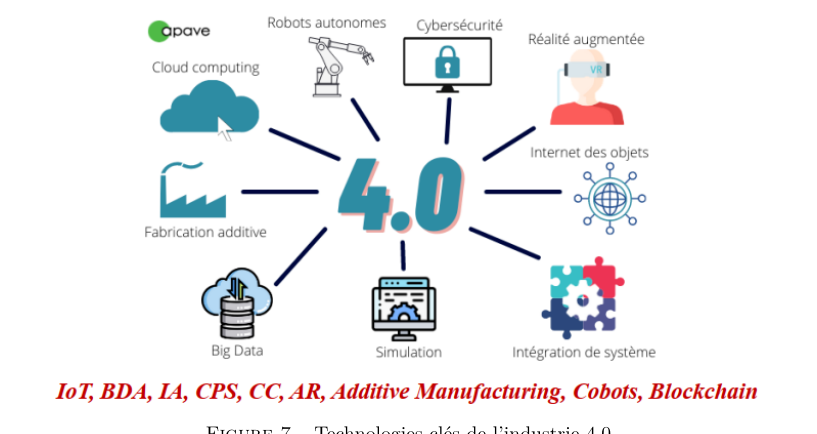
\includegraphics[width=0.65\linewidth]{ch2_technologies_4_0}
\end{center}
\begin{tcolorbox}[colback=white,colframe=bleu,title=Définition,fonttitle=\bfseries]
Une \textbf{usine intelligente} est une usine \textbf{connectée} qui intègre \textbf{processus physiques et processus cyber}.
\end{tcolorbox}
\textbf{Technologies clés :} IoT, Big Data, IA, CPS, Cloud, réalité augmentée (AR), fabrication additive, cobots, blockchain, cybersécurité, simulation, robots autonomes.

\subsection*{3. La pyramide s'aplatit}
\par\begin{Arabic}
التكنولوجيا نضجات. شبكة \textbf{Ethernet} (\fr{RJ45}) كتعوض \textbf{بزاف} ديال الشبكات القديمة، وتقنيات \fr{Web} كتستعمل. الطوابق كيهضرو \textbf{مباشرة} بلا ما يدوزو من طابق لطابق.
\end{Arabic}
\begin{examen}
\begin{itemize}
\item « La pyramide aplatie est un \textbf{concept lié à l'industrie 4.0}. »
\item « Elle a une \textbf{relation directe avec l'avènement de l'internet} / avec le concept Industrie 4.0. »
\item « Elle est due au réseau \textbf{Ethernet} qui remplace de plus en plus les réseaux (terrain), d'usine et de cellules. » \ (test 2023-24 Q38)
\item « Un CPPS est décrit par une \textbf{pyramide productique aplatie}. »
\end{itemize}
\end{examen}
\begin{piege}
\begin{itemize}
\item « Est due à l'utilisation de la \textbf{réalité augmentée} » \faux
\item « Est due à l'utilisation des \textbf{logiciels de gestion de production} » \faux
\item « Est un modèle qui \textbf{met à plat} le système de production » \faux
\item « Est due au réseau Ethernet qui remplace de plus en plus \textbf{les réseaux locaux industriels} » (tous) \faux
\item « Une structure de gestion de la production », « un concept lié à la fabrication additive » \faux
\end{itemize}
\end{piege}
\begin{alerte}
« Ethernet remplace de plus en plus les réseaux \textbf{d'usine et de cellules} » : le \textbf{cours} (§8.3) et le \textbf{test 2023-24 Q38} l'acceptent, mais le \textbf{TD Q34b} le marque faux. \textbf{Décision : on suit le cours et le test (vrai)}, à confirmer avec le prof. Ce qui est faux, c'est de dire qu'il remplace \textbf{tous} les RLI.
\end{alerte}

\subsection*{4. Les CPS (Cyber-Physical Systems)}
\begin{center}
\begin{tabular}{cc}
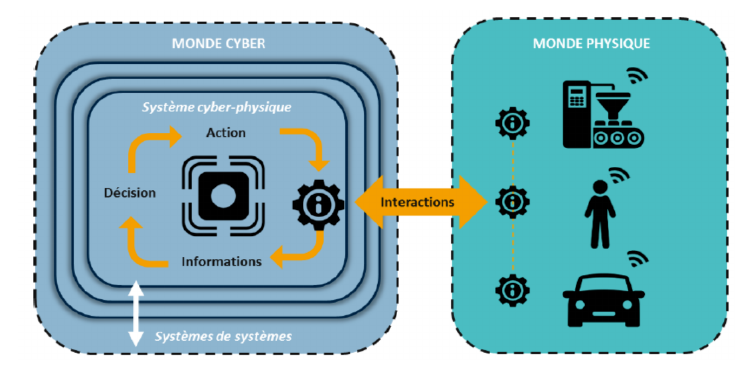
\includegraphics[width=0.46\linewidth]{ch2_cps_monde} &
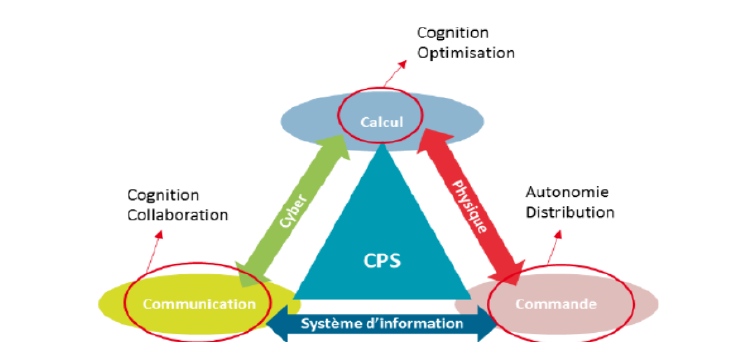
\includegraphics[width=0.46\linewidth]{ch2_cps_piliers}
\end{tabular}
\end{center}
\begin{tcolorbox}[colback=white,colframe=bleu,title=Définition,fonttitle=\bfseries]
Système dans lequel les éléments \textbf{physiques et numériques} interagissent \textbf{en continu} grâce à des flux d'informations \textbf{bidirectionnels}. Les capteurs collectent des données du monde réel, les transmettent à un système informatique qui les analyse et \textbf{renvoie des commandes} aux éléments physiques.
\end{tcolorbox}
\begin{itemize}
\item Des ordinateurs et systèmes embarqués surveillent et contrôlent les processus physiques en \textbf{boucles de rétroaction}.
\item \textbf{Le défi :} doter les objets physiques de capacités de \textbf{communication, perception, action, raisonnement et autonomie}.
\item Les \textbf{3 piliers} : \textbf{Calcul, Communication, Commande}.
\item Nouvelle génération : plus intelligents, mieux connectés, plus adaptatifs et autonomes, avec \textbf{auto-configuration} et \textbf{auto-organisation} ; ils s'appuient sur l'IoT, la réalité augmentée et le Cloud.
\end{itemize}

\begin{examen}
\begin{itemize}
\item « Un CPPS \textbf{intègre des processus physiques et des systèmes informatiques de calcul}. »
\item « Un CPPS est un système de production \textbf{intelligent et connecté}. »
\item « Les CPS sont un \textbf{pilier} de l'industrie 4.0. »
\item « La pyramide aplatie, les CPS, la fabrication additive, la réalité augmentée / virtuelle / mixte, l'intelligence artificielle sont \textbf{tous des concepts liés à l'industrie 4.0}. »
\item « Une usine intelligente \textbf{permet de matérialiser la révolution Industrie 4.0} » et « est \textbf{connectée, intégrant processus physiques et cyber} ».
\item « Le principal objectif de l'Industrie 4.0 : \textbf{productivité et flexibilité à la fois} » et « systèmes de production \textbf{intelligents et autonomes} ».
\item Exemples de CPS : \textbf{drones industriels}, \textbf{dispositifs de santé connectés}, \textbf{bâtiments intelligents} équipés de capteurs, \textbf{systèmes automobiles autonomes}.
\end{itemize}
\end{examen}
\begin{piege}
\begin{itemize}
\item « Un CPPS \textbf{n'a pas de relation avec l'internet} » \faux
\item « Un CPPS \textbf{ne peut être autonome et on ne peut le reconfigurer} » \faux
\item « Un CPPS est un système \textbf{basé sur l'internet des objets} » \faux \quad « entièrement automatisé » \faux
\item « Un CPPS \textbf{consiste en l'utilisation de la réalité augmentée} » \faux \ \ar{(الواقع المعزز كيستعمل فالصيانة)}
\item « Une usine intelligente \textbf{n'est pas un CPS} » \faux \quad « \textbf{n'a pas de relation avec l'IoT} » \faux
\item « Toute usine qui utilise la réalité augmentée » \faux \quad « Toute usine équipée de robots » \faux
\item « Industrie 4.0 est un système de production connecté \textbf{en 4G} » \faux
\item « Appareil électroménager automatique \textbf{sans connectivité} = CPS » \faux
\item « Réduire l'utilisation de l'internet », « minimiser la diversité des produits » \faux
\end{itemize}
\end{piege}

\subsection*{5. Vers l'Industrie 5.0}
Les systèmes de production sont de plus en plus \textbf{autonomes}, \textbf{auto-configurables} et \textbf{auto-organisés}, et permettent la production \textbf{personnalisée et en masse} à la fois. On ajoute \textbf{durabilité, résilience, efficacité} $\Rightarrow$ \textbf{Industrie 5.0}. \textit{(Pas encore tombé aux tests.)}
\begin{center}
\begin{tabularx}{\linewidth}{l X X}
\toprule
& \textbf{Industrie 4.0} & \textbf{Industrie 5.0} \\
\midrule
Focus & \textbf{décision} : technologie, autonomie, connectivité & \textbf{humain} au centre \\
Idée & que peut décider la machine seule ? & comment la technologie sert l'humain et la planète ? \\
Valeurs & efficacité, automatisation & + durabilité et résilience \\
\bottomrule
\end{tabularx}
\end{center}
\textbf{Résilience :} maintenir la productivité malgré les fluctuations (demande, perturbations, environnement). \textbf{Durabilité :} produire en répondant aux besoins actuels sans compromettre ceux des générations futures (environnement, social, économique).

\begin{resume}
\begin{enumerate}
\item Industrie 4.0 = 4\textsuperscript{e} révolution = CPS ; usine intelligente = connectée, physique + cyber.
\item CPS = physique + numérique en interaction continue, 3 piliers Calcul / Communication / Commande ; il a un lien direct avec Internet.
\item Pyramide aplatie = concept Industrie 4.0 grâce à Internet / Ethernet ; elle ne supprime ni ERP ni MES.
\end{enumerate}
\end{resume}

\subsection*{Mini-QCM}
\begin{enumerate}
\item Un CPPS : (a) n'a pas de relation avec l'internet (b) intègre processus physiques et systèmes informatiques de calcul (c) ne peut pas être autonome
\item Une usine intelligente : (a) toute usine avec des robots (b) une usine connectée intégrant processus physiques et cyber
\item Un exemple de CPS : (a) un drone industriel connecté (b) un appareil électroménager sans connectivité
\item La pyramide aplatie : (a) due à la réalité augmentée (b) liée à l'Industrie 4.0 et à l'avènement d'Internet
\item Les 3 piliers du CPS : (a) Calcul, Communication, Commande (b) Capteur, Contrôle, Cloud
\end{enumerate}
{\small\textit{Réponses : 1-b, 2-b, 3-a, 4-b, 5-a.}}

%======================================================================
\partie{Bilan du chapitre 2 : à relire la veille de l'examen}

\subsection*{Top 12 des pièges du chapitre 2}
\begin{enumerate}
\item « Un FMS produit \textbf{une seule variante} », « sans supervision humaine » $\rightarrow$ FAUX.
\item Cellule flexible $\neq$ lignes de transfert ; atelier flexible \textbf{plus flexible} que la cellule.
\item La pyramide CIM a \textbf{5 niveaux} (0 à 4) : capteurs, automates, SCADA, MES, ERP.
\item Le \textbf{réseau de cellule} relie automates $\leftrightarrow$ SCADA (pas les capteurs).
\item CANopen et AS-i : niveau \textbf{A} ; Ethernet Modbus TCP : niveaux \textbf{B, C, D}.
\item MES = \textbf{ordonnancement détaillé, traçabilité, OF} ; il ne « supervise » pas (tests).
\item SCADA = supervision, collecte des données ; ERP = finances, logistique, RH.
\item ERP ne fait \textbf{pas} la planification détaillée (c'est le MES).
\item Plug and Produce : \textbf{standards universels}, interopérabilité ; jamais « propriétaire ».
\item Intégré $\not\Rightarrow$ reconfigurable (mais reconfigurable $\Rightarrow$ intégré).
\item CPS : \textbf{lien avec Internet}, autonome et reconfigurable ; ni « réalité augmentée » ni « IoT seulement ».
\item Pyramide aplatie : lien direct avec Internet / Industrie 4.0 ; ne supprime \textbf{pas} ERP et MES.
\end{enumerate}

\subsection*{Conflits à confirmer avec le prof}
\begin{itemize}
\item MES et « superviser en temps réel » (TD vrai, test faux).
\item « Aléas » : SCADA (TD) ou MES (cours) ?
\item Pyramide aplatie : Ethernet remplace les réseaux d'usine et de cellules (cours et test vrai, TD faux).
\item Cellule flexible : « $n=1$ à $4$ machines CNC » (test) vs « plusieurs » (cours).
\end{itemize}

\subsection*{Checklist}
\begin{itemize}[label=$\square$]
\item Je connais les 5 composants du FMS et la différence ligne de transfert / cellule / atelier / MOCN.
\item Je sais les 5 niveaux de la pyramide CIM, du bas vers le haut.
\item Je sais placer les 4 réseaux (terrain, cellule, atelier, usine) entre les niveaux.
\item Je sais remplir le tableau A--E avec les protocoles (CANopen, AS-i, Ethernet Modbus TCP).
\item Je distingue SCADA, MES et ERP et je connais le dialogue ERP--MES--atelier.
\item Je connais Plug and Produce et la différence FMS / RMS.
\item Je sais définir un CPS, une usine intelligente et la pyramide aplatie.
\item Je connais les exemples de CPS et les phrases fausses sur l'IoT, la réalité augmentée, la 4G.
\end{itemize}


\end{document}
